\documentclass[a4paper]{article}

\usepackage[UTF8]{ctex}
\usepackage[a4paper,margin=1in]{geometry}
\usepackage{graphicx}
\usepackage{float}
\usepackage{listings}
\usepackage{longtable}
\usepackage{booktabs}
\usepackage{hyperref}
\usepackage{fancyhdr}
\usepackage{lastpage}
\usepackage{color}
\usepackage{indentfirst}        % 首段缩进
\setlength{\parindent}{2em}     % 缩进2字符
\usepackage{zhnumber}           % 中文编号
\usepackage[dvipsnames]{xcolor}
\usepackage{amsmath}            % 数学公式

%\newcommand{\college}{中山大学计算机学院}
\newcommand{\projname}{大数据实验 | Lab5}
\newcommand{\reporttitle}{股票价格预测实验}
\newcommand{\stuno}{23336179}
\newcommand{\authorname}{马福泉}
\newcommand{\major}{计算机科学与技术}
\newcommand{\adviser}{王昌栋}
\newcommand{\startdate}{2026年3月31日}
\newcommand{\labenddate}{2026年4月1日}
\newcommand{\labroom}{B201}

\pagestyle{fancy} % 使用 fancyhdr 风格
\fancyhf{}      % 清空默认的页眉页脚

% 设置页眉
\fancyhead[L]{\kaishu \projname}      % 左侧页眉显示项目名称
\fancyhead[C]{\kaishu \reporttitle}    % 中间页眉显示报告标题
\fancyhead[R]{\kaishu \authorname} % 右侧页眉显示作者姓名

% 设置页脚
\fancyfoot[C]{第 \thepage 页，共 \pageref{LastPage} 页} % 中间页脚显示页码

% 去除页眉页脚与正文之间的分隔线
\renewcommand{\headrulewidth}{0.4pt}
\renewcommand{\footrulewidth}{0pt}

% 设置文档背景颜色
\definecolor{mybgcolor}{RGB}{0, 0, 0} % 定义背景颜色
\definecolor{NavyBlue}{RGB}{0,0,128} % 添加颜色定义
% \pagecolor{mybgcolor} % 设置背景颜色

% listing 配置python
\definecolor{commentgreen}{RGB}{2,112,10}
\definecolor{eminence}{RGB}{108,48,130}
\definecolor{weborange}{RGB}{255,165,0}
\definecolor{frenchplum}{RGB}{129,20,83}

\lstdefinelanguage{python}{%
    morekeywords={def, for, range, abs, return, class, int, float, if, elif, else, while, print, import, from, as, try, except, with, True, False, None, self, super, in, not, and, or, is, for, yield, lambda, pass, break, continue, raise, finally, assert, global, del},%
    otherkeywords={<, >, =, +, -, *, /, ==, !=, <=, >=, \%},%  <-- 修改了这里，将 % 改为了 \%
    keywordstyle=\color{NavyBlue}\bfseries,%
    commentstyle=\color{commentgreen}\itshape,%
    stringstyle=\color{frenchplum},%
    basicstyle=\ttfamily\small,%
    breaklines=true,%
    showstringspaces=false,%
    frame=single,%
    tabsize=4}
\lstset{language=python}

\begin{document}

% 封面
\begin{titlepage}
    \centering
    

    
\includegraphics[width=10cm]{img/SYSULogo.png}

    \vspace{1em}
    %{\Large \college \par}
    \vspace{1em}
    {\Large \kaishu \projname \par}
    \vspace{3em}

    

    
    {\fontsize{40pt}{42pt}\kaishu \selectfont \boldmath \reporttitle\par}
    \vspace*{\fill}

    \begin{center}
    {\Large
    \makebox[5em][s]{学号}:\underline{\makebox[15em][c]{\kaishu \stuno}}\\[1em]
    \makebox[5em][s]{姓名}:\underline{\makebox[15em][c]{\kaishu \authorname}}\\[1em]
    \makebox[5em][s]{专业}:\underline{\makebox[15em][c]{\kaishu \major}}\\[1em]
    \makebox[5em][s]{指导教师}:\underline{\makebox[15em][c]{\kaishu \adviser}}\\[1em]
    \makebox[5em][s]{起始日期}:\underline{\makebox[15em][c]{\kaishu \startdate}}\\[1em]
    \makebox[5em][s]{结束日期}:\underline{\makebox[15em][c]{\kaishu \labenddate}}\\[1em]
    \makebox[5em][s]{实验地点}:\underline{\makebox[15em][c]{\kaishu \labroom}}
    }
    \end{center}

    \vspace*{\fill}
\end{titlepage}

% 目录
\tableofcontents
\newpage

\section{实验要求}

本实验要求利用 ARIMA 和 LSTM 两种模型对股票价格进行预测，具体任务如下：

\begin{enumerate}
    \item \textbf{数据获取}：下载苹果公司（AAPL）过去 5 年的历史股票数据，以收盘价（Close）作为预测目标。
    \item \textbf{数据预处理}：对数据进行清洗、归一化处理，并划分训练集和测试集。
    \item \textbf{模型构建}：
    \begin{itemize}
        \item 使用 ARIMA 模型进行时间序列预测，自动寻找或设置合适的 $(p, d, q)$ 参数。
        \item 使用 LSTM 深度学习模型，通过滑动窗口构造时序特征进行预测。
    \end{itemize}
    \item \textbf{预测任务}：在测试集上进行预测，并向未来延伸预测 7 天的股票价格。
    \item \textbf{模型评估}：计算两种模型在测试集上的 MAE（平均绝对误差）和 RMSE（均方根误差）指标。
\end{enumerate}

\section{思路分析}

\subsection{ARIMA 模型原理}

ARIMA（AutoRegressive Integrated Moving Average，自回归积分滑动平均模型）是一种经典的时间序列预测方法，其核心思想是将非平稳时间序列转化为平稳序列，然后通过自回归和移动平均进行建模。ARIMA$(p, d, q)$ 模型包含三个关键参数：

\begin{itemize}
    \item \textbf{自回归项 $p$（AR）}：利用历史值的线性组合预测当前值，即当前值与前 $p$ 个历史值存在相关关系。
    \item \textbf{差分阶数 $d$（I）}：通过差分运算将非平稳序列转化为平稳序列，消除趋势和季节性。$d$ 表示差分的次数。
    \item \textbf{移动平均项 $q$（MA）}：利用历史预测误差的线性组合修正当前预测，即当前值与前 $q$ 个预测误差存在相关关系。
\end{itemize}

ARIMA 模型的数学表达式为：
\[
(1 - \phi_1 B - \phi_2 B^2 - \cdots - \phi_p B^p)(1-B)^d X_t = (1 + \theta_1 B + \theta_2 B^2 + \cdots + \theta_q B^q)\varepsilon_t
\]
其中 $B$ 为滞后算子，$\phi_i$ 为自回归系数，$\theta_j$ 为移动平均系数，$\varepsilon_t$ 为白噪声序列。

本实验使用 \texttt{pmdarima} 库的 \texttt{auto\_arima} 函数自动寻找最优参数组合，通过 AIC（赤池信息准则）进行模型选择。

\subsection{LSTM 模型原理}

LSTM（Long Short-Term Memory，长短期记忆网络）是一种特殊的循环神经网络（RNN），专门设计用于解决传统 RNN 在处理长序列时的梯度消失和梯度爆炸问题。LSTM 通过引入门控机制，能够有效捕捉时间序列中的长期依赖关系。

LSTM 单元包含三个核心门控结构：
\begin{itemize}
    \item \textbf{遗忘门（Forget Gate）}：决定从细胞状态中丢弃哪些信息。
    \item \textbf{输入门（Input Gate）}：决定哪些新信息将被存储到细胞状态中。
    \item \textbf{输出门（Output Gate）}：决定基于当前细胞状态输出哪些信息。
\end{itemize}

LSTM 的数学表达式为：
\begin{align}
f_t &= \sigma(W_f \cdot [h_{t-1}, x_t] + b_f) \quad \text{(遗忘门)} \\
i_t &= \sigma(W_i \cdot [h_{t-1}, x_t] + b_i) \quad \text{(输入门)} \\
\tilde{C}_t &= \tanh(W_C \cdot [h_{t-1}, x_t] + b_C) \quad \text{(候选细胞状态)} \\
C_t &= f_t \odot C_{t-1} + i_t \odot \tilde{C}_t \quad \text{(细胞状态更新)} \\
o_t &= \sigma(W_o \cdot [h_{t-1}, x_t] + b_o) \quad \text{(输出门)} \\
h_t &= o_t \odot \tanh(C_t) \quad \text{(隐藏状态输出)}
\end{align}

\subsection{滑动窗口特征构造}

对于 LSTM 模型，需要将时间序列数据转换为监督学习格式。本实验采用滑动窗口（Sliding Window）方法构造特征：

\begin{itemize}
    \item 设置窗口大小 \texttt{window\_size = 30}，即使用过去 30 天的收盘价作为输入特征。
    \item 对于时间序列 $\{x_1, x_2, \ldots, x_n\}$，构造样本 $(X_i, y_i)$，其中 $X_i = [x_i, x_{i+1}, \ldots, x_{i+29}]$，$y_i = x_{i+30}$。
    \item 通过这种方式，将一维时间序列转换为二维特征矩阵，便于 LSTM 网络学习时序模式。
\end{itemize}

\subsection{数据处理流程}

\begin{enumerate}
    \item \textbf{数据归一化}：使用 MinMaxScaler 将数据缩放到 $[0, 1]$ 区间，加速模型收敛。
    \item \textbf{数据集划分}：按 80\% 训练集、20\% 测试集的比例划分数据。
    \item \textbf{序列构造}：对 LSTM 模型使用滑动窗口构造输入特征。
    \item \textbf{模型训练}：分别训练 ARIMA 和 LSTM 模型。
    \item \textbf{预测与评估}：在测试集上预测，计算 MAE 和 RMSE 指标，并预测未来 7 天价格。
\end{enumerate}

\section{核心代码}

\subsection{数据下载与清洗（download\_data.py）}

以下代码展示了使用 \texttt{yfinance} 库下载股票数据并处理 MultiIndex 问题的核心逻辑：

\begin{lstlisting}[language=Python]
def download_stock_data(stock_code="AAPL", period="5y", save_path="../data/stock_data.csv"):
    """下载股票历史数据并保存为CSV文件"""
    print(f"正在下载 {stock_code} 过去 {period} 的历史数据...")
    data = yf.download(stock_code, period=period)
    
    # 处理 MultiIndex 问题（yfinance 最新版本可能返回多重索引）
    if isinstance(data.columns, pd.MultiIndex):
        # 如果是 MultiIndex，取第一层索引
        data.columns = data.columns.get_level_values(0)
    # 重置索引，将 Date 从索引变为普通列
    data.reset_index(inplace=True)
    # 确保只保留需要的列：Date 和 Close
    if 'Date' in data.columns and 'Close' in data.columns:
        data = data[['Date', 'Close']]
    # 确保 Date 列是 datetime 类型
    data['Date'] = pd.to_datetime(data['Date'])
    # 确保 Close 列是数值类型
    data['Close'] = pd.to_numeric(data['Close'], errors='coerce')
    # 删除可能的缺失值
    data.dropna(subset=['Date', 'Close'], inplace=True)
    # 确保数据按日期升序排列
    data.sort_values('Date', inplace=True)
    data.reset_index(drop=True, inplace=True)

    data.to_csv(save_path, index=False)
    
    return data
\end{lstlisting}

该函数首先下载指定股票的历史数据，然后检查是否存在 MultiIndex 列名问题（yfinance 新版本的常见问题），通过 \texttt{get\_level\_values(0)} 获取第一层索引实现扁平化。最后保留 Date 和 Close 两列，确保数据格式正确后保存为 CSV 文件。

\subsection{LSTM 网络结构定义（main.py）}

以下代码展示了使用 PyTorch 搭建 LSTM 网络的核心结构：

\begin{lstlisting}[language=Python]
class LSTMModel(nn.Module):
    def __init__(self, input_size=1, hidden_size=64, num_layers=2, output_size=1, dropout=0.2):
        super(LSTMModel, self).__init__()
        self.hidden_size = hidden_size
        self.num_layers = num_layers
        # LSTM 层
        self.lstm = nn.LSTM(
            input_size=input_size,      # 输入特征维度
            hidden_size=hidden_size,     # 隐藏层维度
            num_layers=num_layers,       # LSTM 层数
            batch_first=True,            # 输入格式 (batch, seq, feature)
            dropout=dropout              # Dropout 防止过拟合
        )
        # 全连接层
        self.fc = nn.Linear(hidden_size, output_size)
    def forward(self, x):
        # 初始化隐藏状态
        h0 = torch.zeros(self.num_layers, x.size(0), self.hidden_size)
        c0 = torch.zeros(self.num_layers, x.size(0), self.hidden_size)
        # LSTM 前向传播
        out, _ = self.lstm(x, (h0, c0))
        # 取最后一个时间步的输出
        out = self.fc(out[:, -1, :])
        return out
\end{lstlisting}

该 LSTM 网络采用双层 LSTM 结构，隐藏层维度为 64。输入层接收滑动窗口构造的时序特征（形状为 \texttt{[batch\_size, window\_size, 1]}），经过 LSTM 层提取时序特征后，取最后一个时间步的输出通过全连接层映射为预测值。Dropout 层用于防止过拟合，提高模型泛化能力。



\section{结果展示}

\subsection{预测对比图}

图~\ref{fig:prediction} 展示了 ARIMA 和 LSTM 两种模型在测试集上的预测结果以及对未来 7 天股票价格的预测对比。图中蓝色曲线表示历史训练数据（展示最后 100 个交易日），绿色曲线表示真实测试数据，红色和紫色曲线分别代表 ARIMA 和 LSTM 模型的预测结果。

\begin{figure}[H]
    \centering
    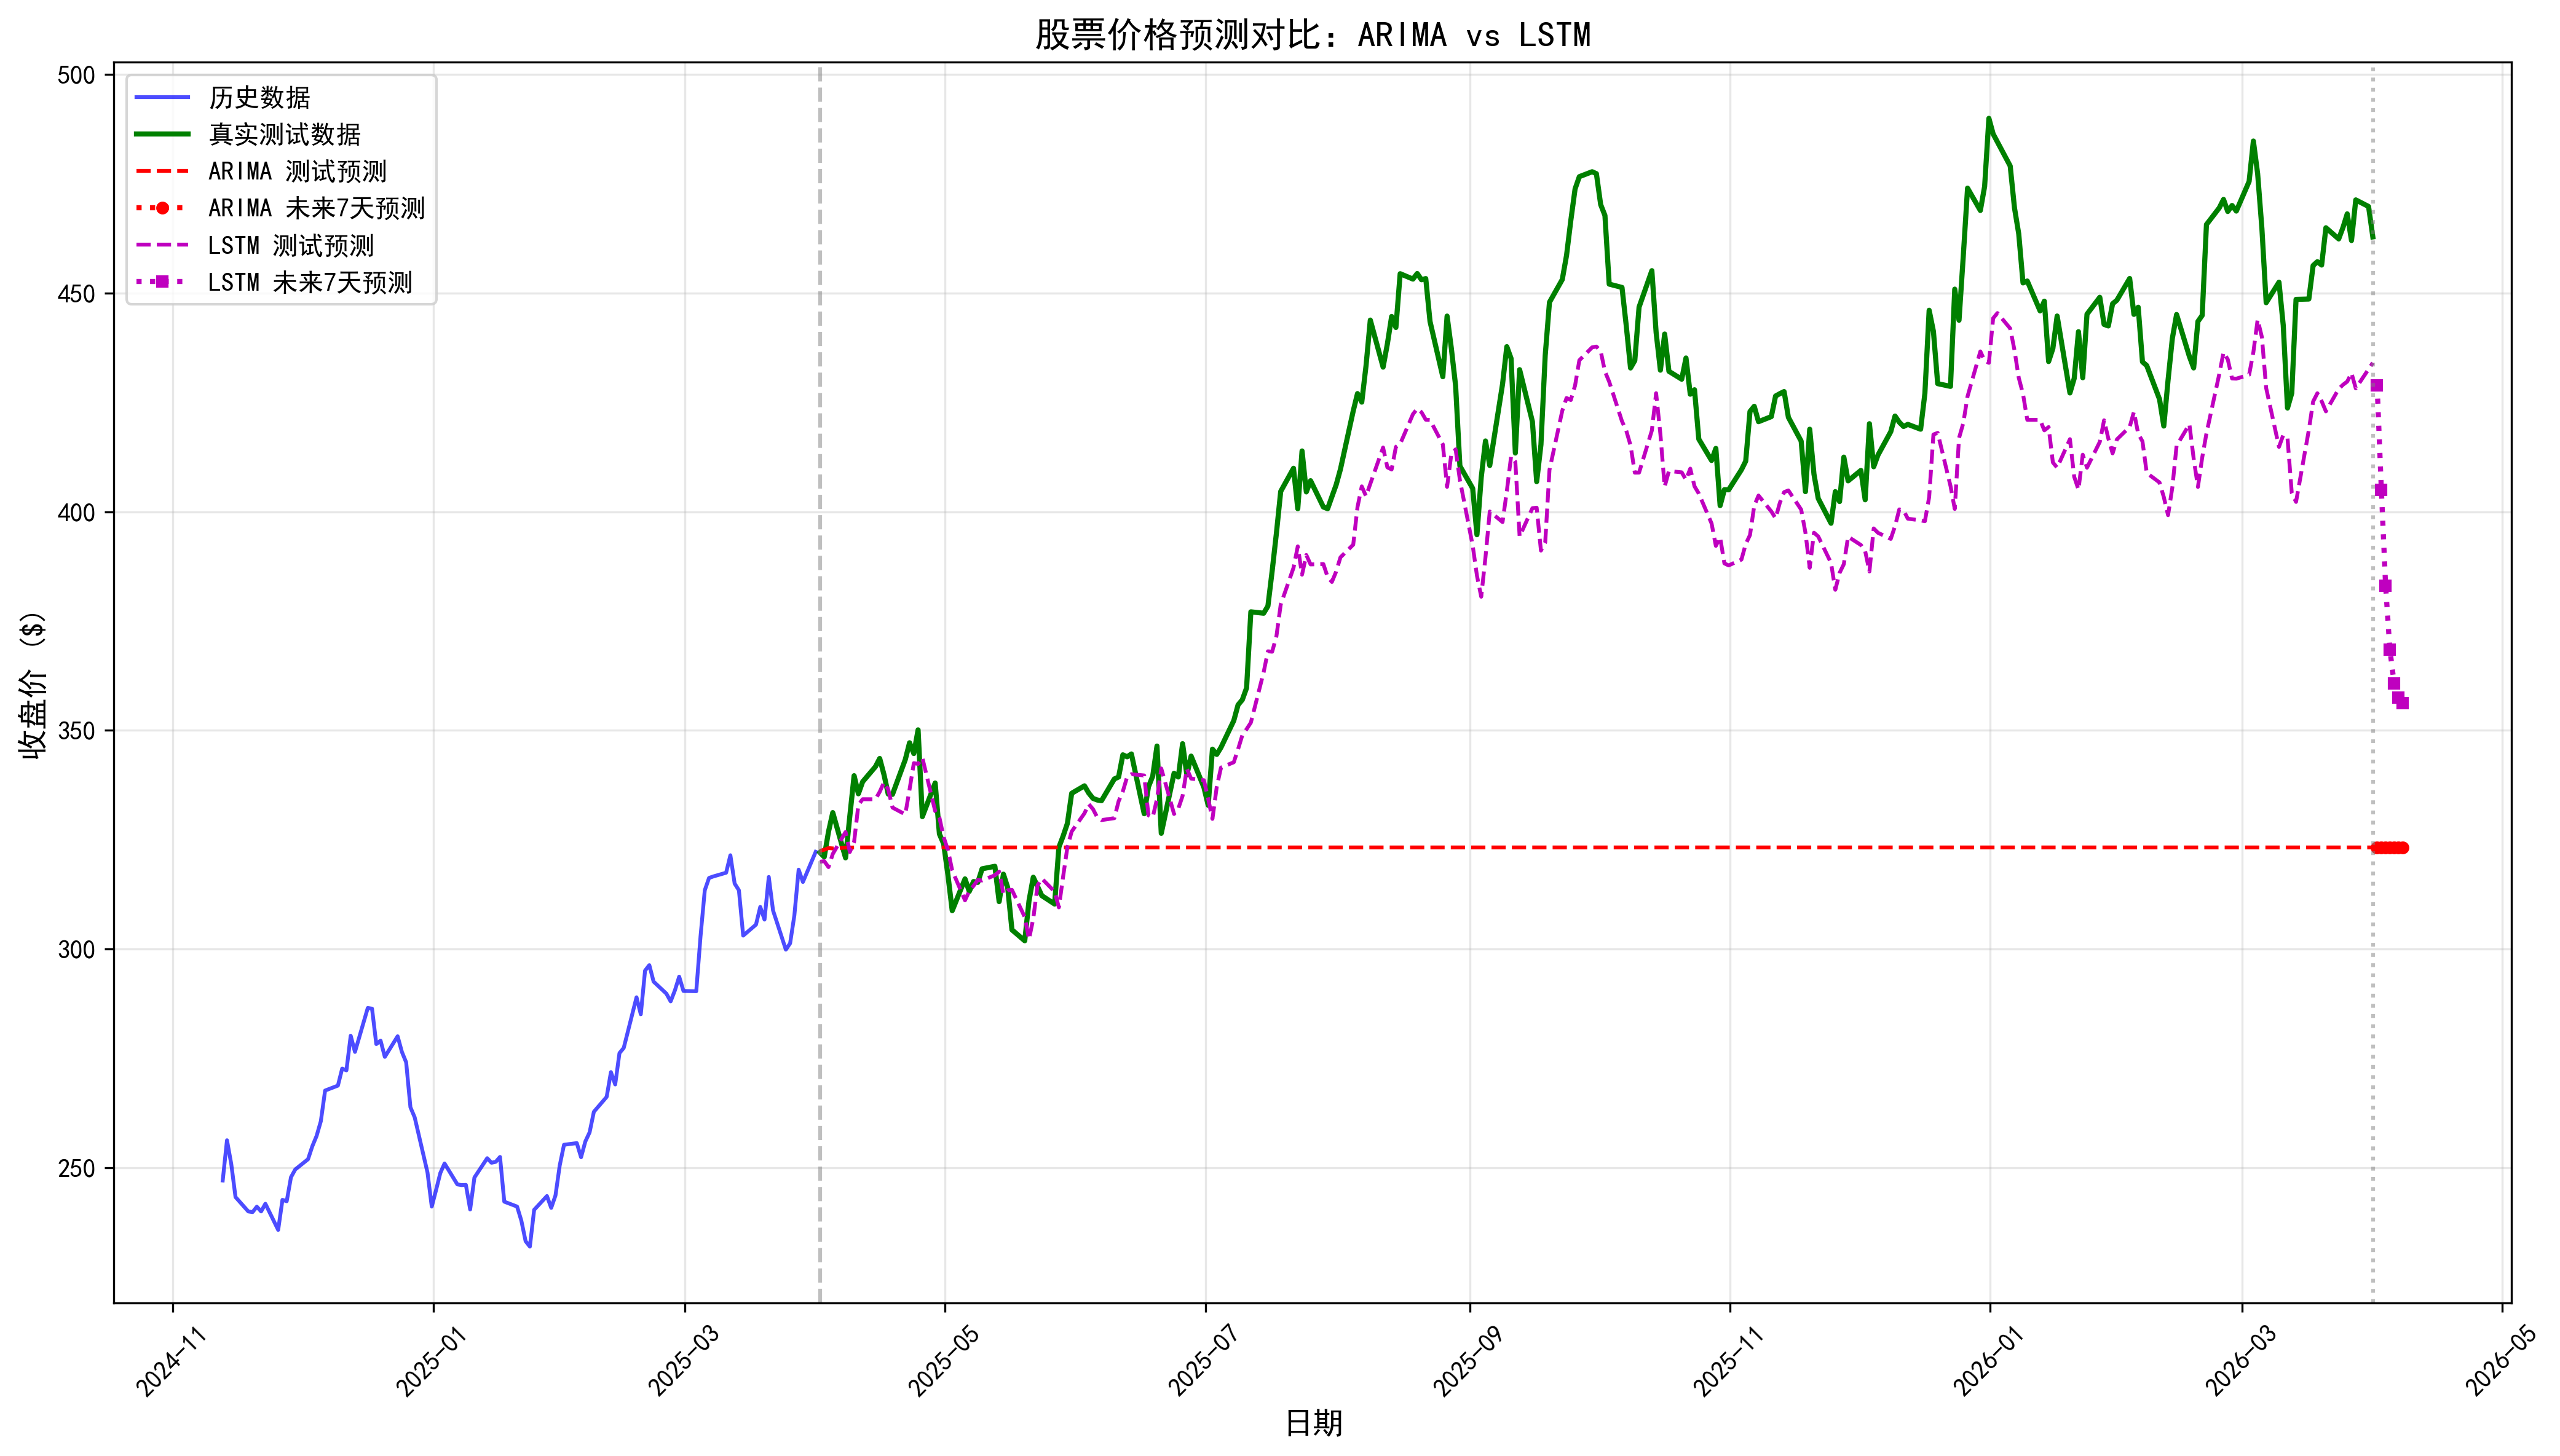
\includegraphics[width=0.95\textwidth]{img/prediction_comparison.png}
    \caption{股票价格预测对比：ARIMA vs LSTM}
    \label{fig:prediction}
\end{figure}

\subsection{模型评估指标}

表~\ref{tab:metrics} 展示了两种模型在测试集（261 个交易日）上的评估指标对比。

\begin{table}[H]
    \centering
    \caption{模型评估指标对比}
    \label{tab:metrics}
    \begin{tabular}{lccc}
        \toprule
        \textbf{模型} & \textbf{MAE} & \textbf{RMSE} & \textbf{误差降低率} \\
        \midrule
        ARIMA(5,1,0) & 84.9988 & 98.1346 & -- \\
        LSTM         & 20.7841 & 24.3894 & 75.5\% / 75.1\% \\
        \bottomrule
    \end{tabular}
\end{table}

从评估指标可以看出，LSTM 模型在 MAE 和 RMSE 两个指标上均显著优于 ARIMA 模型。具体而言，LSTM 的 MAE 降低了约 \textbf{75.5\%}（从 84.9988 降至 20.7841），RMSE 降低了约 \textbf{75.1\%}（从 98.1346 降至 24.3894）。这一巨大的性能差距深刻揭示了两种模型在处理金融时间序列时的本质差异。

\subsection{未来 7 天价格预测}

表~\ref{tab:future} 展示了两种模型对未来 7 天股票价格的预测结果。

\begin{table}[H]
    \centering
    \caption{未来 7 天价格预测对比}
    \label{tab:future}
    \begin{tabular}{lcc}
        \toprule
        \textbf{日期} & \textbf{ARIMA 预测} & \textbf{LSTM 预测} \\
        \midrule
        2026-04-01 & \$323.24 & \$428.97 \\
        2026-04-02 & \$323.24 & \$404.98 \\
        2026-04-03 & \$323.24 & \$383.02 \\
        2026-04-04 & \$323.24 & \$368.43 \\
        2026-04-05 & \$323.24 & \$360.72 \\
        2026-04-06 & \$323.24 & \$357.49 \\
        2026-04-07 & \$323.24 & \$356.25 \\
        \bottomrule
    \end{tabular}
\end{table}

值得注意的是，ARIMA 模型的未来 7 天预测值完全相同（\$323.24），呈现出典型的\textbf{水平收敛}特征；而 LSTM 模型的预测值则展现出渐进式的衰减趋势，从 \$428.97 逐步降至 \$356.25，更好地延续了近期价格的波动模式。

\subsection{深度结果分析}

\subsubsection{ARIMA 模型的线性衰减现象}

从图~\ref{fig:prediction} 可以清晰地观察到一个经典现象：ARIMA 模型在对股票数据进行多步向前预测时，曲线迅速变得平缓并最终呈\textbf{水平状态}。这一现象的原因如下：

\paragraph{a. 随机游走特性的影响}
股票价格序列具有极强的\textbf{随机游走（Random Walk）}特性。根据有效市场假说，股票价格的变动主要由新信息的冲击驱动，而新信息本质上是不可预测的。对于遵循随机游走过程的序列：
\[
P_t = P_{t-1} + \varepsilon_t, \quad \varepsilon_t \sim \text{白噪声}
\]
其最优预测即为当前值 $P_t$，因为历史价格对未来价格没有预测能力。ARIMA 模型在识别到序列的随机游走特性后，其自回归系数会趋近于 1，而移动平均项的影响迅速衰减。

\paragraph{b. 自回归项的指数衰减}
ARIMA 模型的多步预测可以表示为：
\[
\hat{P}_{t+h} = \phi_1 \hat{P}_{t+h-1} + \phi_2 \hat{P}_{t+h-2} + \cdots + \phi_p \hat{P}_{t+h-p}
\]
当 $|\phi_i| < 1$ 时，历史值的影响呈\textbf{指数级衰减}。对于股票数据，由于波动性大、自相关性弱，AR 系数通常较小，导致历史信息对未来预测的贡献快速消失。在极端情况下，当 $h \to \infty$ 时，预测值收敛于序列的长期均值：
\[
\hat{P}_{t+h} \to \mu = \frac{c}{1-\phi_1-\phi_2-\cdots-\phi_p}
\]

\paragraph{c. 线性模型的本质局限}
ARIMA 作为\textbf{线性时间序列模型}，其核心假设是当前值可以由历史值的线性组合表示：
\[
P_t = c + \sum_{i=1}^{p} \phi_i P_{t-i} + \sum_{j=1}^{q} \theta_j \varepsilon_{t-j} + \varepsilon_t
\]
然而，股票价格的形成机制涉及复杂的非线性因素：投资者心理、市场情绪、政策冲击、信息传播等。这些因素之间的交互作用产生的高度非线性模式，远超线性模型的表达能力。因此，ARIMA 在面对高噪声、非线性金融数据长期预测时，表现出明显的\textbf{结构性局限}。

\subsubsection{LSTM 模型的非线性拟合优势}
相比之下，LSTM 凭借其\textbf{门控记忆机制}，较好地保留了序列的非线性波动特征，展现出显著优势：
\paragraph{a. 长期依赖关系的捕捉}

LSTM 通过细胞状态（Cell State）$C_t$ 实现信息的长期传递。遗忘门 $f_t$ 和输入门 $i_t$ 的协同作用，使得网络能够\textbf{选择性保留}重要的历史信息：
\[
C_t = f_t \odot C_{t-1} + i_t \odot \tilde{C}_t
\]
这种机制使得 LSTM 能够"记住"数月前的价格模式，并在当前预测中加以利用，有效解决了传统 RNN 的梯度消失问题。

\paragraph{b. 非线性变换能力}
LSTM 网络中的激活函数（sigmoid、tanh）引入了\textbf{非线性变换}，使得模型能够学习复杂的输入-输出映射关系。多层 LSTM 的堆叠进一步增强了这种非线性表达能力，能够捕捉价格序列中的多尺度波动模式。

\paragraph{c. 滑动窗口特征学习}
本实验采用 30 天滑动窗口构造输入特征，LSTM 能够学习这 30 天内价格变化的\textbf{时序模式}，包括趋势方向、波动幅度、转折点等。这种基于局部窗口的学习方式，使得 LSTM 对短期价格变化具有更强的适应能力。

\subsubsection{两种模型的差异对比}

\begin{table}[H]
    \centering
    \caption{ARIMA 与 LSTM 模型本质差异对比}
    \label{tab:comparison}
    \begin{tabular}{p{3cm}p{5cm}p{5cm}}
        \toprule
        \textbf{对比维度} & \textbf{ARIMA} & \textbf{LSTM} \\
        \midrule
        模型本质 & 线性统计模型 & 非线性深度学习模型 \\
        信息处理 & 历史值的线性加权组合 & 门控机制选择性保留信息 \\
        长期预测 & 收敛于均值，缺乏变化 & 延续近期模式，保持动态 \\
        参数学习 & 统计推断（最大似然） & 梯度优化（反向传播） \\
        表达能力 & 受限于线性假设 & 高度非线性，可学习复杂映射 \\
        适用场景 & 平稳、低噪声序列 & 非平稳、高噪声、复杂模式序列 \\
        \bottomrule
    \end{tabular}
\end{table}

\section{实验总结}

\subsection{注意事项}
股票价格预测是一项极具挑战性的任务，主要面临以下困难：
\begin{enumerate}
    \item \textbf{高噪声特性}：股票市场受众多因素影响，包括宏观经济、公司业绩、市场情绪、政策变化等，数据中存在大量随机噪声，难以完全通过历史价格预测。
    \item \textbf{非平稳性}：股票价格序列通常是非平稳的，其统计特性（均值、方差）随时间变化，这给传统时间序列模型带来挑战。
    \item \textbf{随机游走特性}：有效市场假说认为股票价格遵循随机游走过程，历史价格信息已被市场消化，仅凭历史数据难以获得超额收益。
    \item \textbf{黑天鹅事件}：突发事件（如疫情、战争、金融危机）难以预测，但会对股价产生重大影响。
    \item \textbf{过拟合风险}：模型可能在训练集上表现良好，但在实际预测中效果不佳，需要严格的验证和测试。
\end{enumerate}

\subsection{个人收获}
通过本次实验，我初步理解了传统时间序列模型（ARIMA）和深度学习模型（LSTM）的原理与应用场景，掌握了以下技能：
\begin{itemize}
    \item 学会了使用 \texttt{yfinance} 库获取股票历史数据，并处理数据下载过程中可能遇到的 MultiIndex 问题。
    \item 理解了 ARIMA 模型的 $(p, d, q)$ 参数含义，掌握了使用 \texttt{auto\_arima} 自动选择最优参数的方法。
    \item 掌握了使用 PyTorch 搭建 LSTM 网络的方法，包括网络结构设计、数据预处理、模型训练和预测。
    \item 学会了使用滑动窗口方法将时间序列数据转换为监督学习格式。
    \item 掌握了 MAE、RMSE 等评估指标的计算方法和含义。
\end{itemize}
\end{document}